\newenvironment{ebnf}
  {\newcommand{\NTerm}[1]{##1}
   \newcommand{\Rule}[2]{\item[##1]
        ::=\; ##2}
   \newcommand{\OrRule}[1]{\par
        \ \ \ \textbar\ ##1 }
   \newcommand{\Token}[1]{\mbox{\small{`\textsf{\textbf{##1}}'}}}
   \newcommand{\ZeroOrMore}[1]{{##1}*}
   \newcommand{\OneOrMore}[1]{{##1}+}
   \newcommand{\OrList}[1]{(\ ##1\ )}
   \newcommand{\OrSep}{\ \textbar\ }
   \newcommand{\Optional}[1]{{##1}?}
   \begin{flushleft}
   \begin{list}{}{
     \unboldmath
     \setlength{\parsep}{0cm}
     \setlength{\itemsep}{0cm}
     \setlength{\parskip}{0cm}
     \renewcommand{\makelabel}[1]{##1\hfil}
     \setlength{\labelwidth}{2cm}
     \setlength{\leftmargin}{3cm}
%     \settowidth{\itemindent}{::= \;\;\;}
%     \setlength{\itemindent}{0cm}
%     \settowidth{\listparindent}{\textbar \;\;\;\;}
%     \setlength{\listparindent}{0pt - \listparindent}
%     \setlength{\leftmargin}{\labelwidth + \labelsep - \itemindent}
}
   \begin{sloppypar}}
   {\end{sloppypar}\end{list}\end{flushleft}}

\begin{nestedsection}{R4: Rule-based Reasoning over RDF streams using Rete}{implementation}
	As a proof of concept, we have implemented R4: a Rule-based Reasoner for RDF-streams using Rete.
	Reasoning in R4 is performed continuously and incrementally as dataflow networks that work directly on RDF streams.
	The system architecture is shown in \reffig{R4-architecture}.
	\begin{figure}[t]
		\centering
		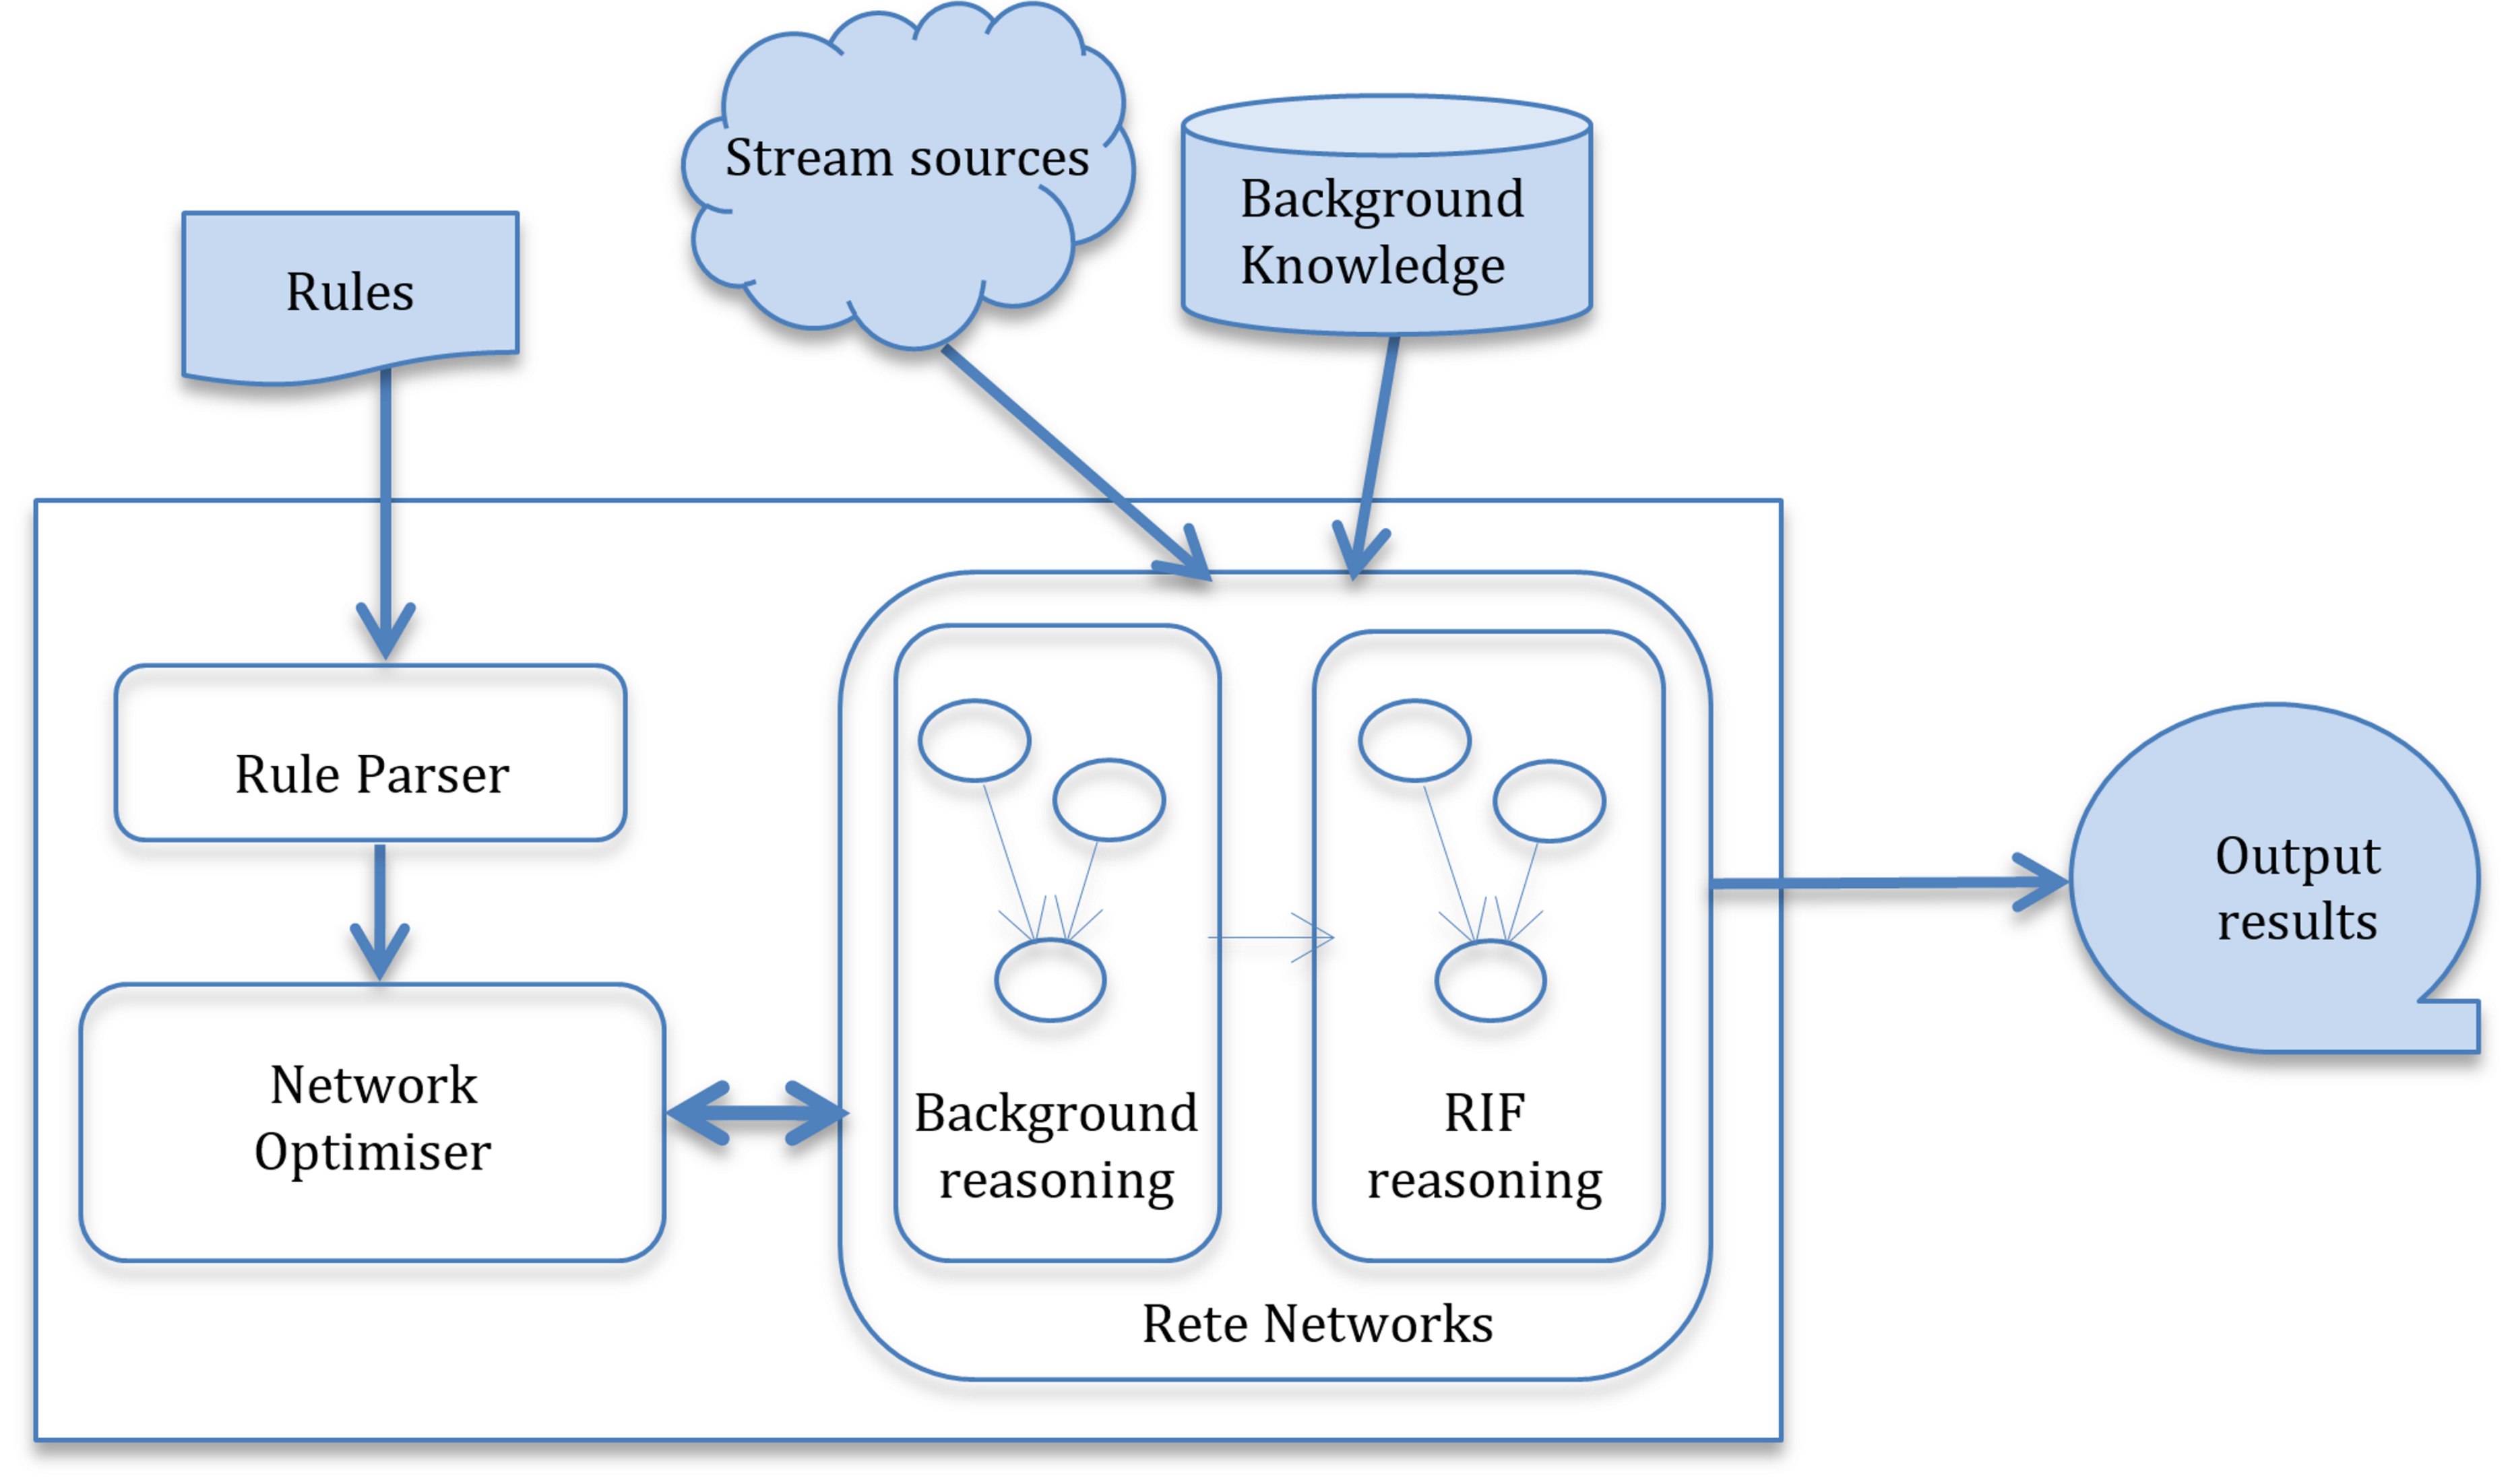
\includegraphics[width=0.45\textwidth]{R4-architecture}
		\caption{The system architecture of R4.}
		\labelfig{R4-architecture}
	\end{figure}

	A rule document containing any number of rules is submitted to the system.
	We have chosen RIF-Core to be the language in which rules can be represented, for being compatible with RDF and other semantic web standards.
	The rule document specifies any domain-specific rules as well as an entailment regime \emph{if any} for background reasoning.
	We also added a simple extension to RIF-Core to enable users to specify window constraints as part of their rules, as shown in Listing~\ref{lst-S-RIF-Core}.

\begin{figure*}
\begin{ebnf}
\Rule{Document}{
        \Optional{\NTerm{IRIMETA}} 
        \Token{Document} 
        \Token{(} 
        \Optional{\NTerm{Base}} 
        \ZeroOrMore{\NTerm{Prefix}} 
        \ZeroOrMore{\NTerm{Import}} 
        \Optional{\NTerm{Group}} 
        \Token{)}
}
\Rule{Base}{
        \Token{Base} 
        \Token{(} 
        \NTerm{ANGLEBRACKIRI} 
        \Token{)}
}
\Rule{Prefix}{
        \Token{Prefix} 
        \Token{(} 
        \NTerm{Name} 
        \NTerm{ANGLEBRACKIRI} \Token{)}
}
\Rule{Import}{
        \Optional{\NTerm{IRIMETA}} 
        \Token{Import} 
        \Token{(} 
        \NTerm{LOCATOR} 
        \Optional{\NTerm{PROFILE}} 
        \Token{)}
}
\Rule{Group}{
        \Optional{\NTerm{IRIMETA}} 
        \Token{Group} 
        \Token{(} 
        \ZeroOrMore{\OrList{\NTerm{RULE} \OrSep \NTerm{Group}}} 
        \Token{)}
}
\Rule{RULE}{
        \Optional{\NTerm{IRIMETA}}
        \Token{Forall}
        \OneOrMore{\NTerm{Variable}}
        \Token{(}
        \NTerm{CLAUSE}
        \Token{)}
}
\OrRule{
        \NTerm{CLAUSE}
}
\Rule{CLAUSE}{
        \OrList{\NTerm{Implies} \OrSep \NTerm{ATOMIC}}
}
\Rule{Implies}{
        \Optional{\NTerm{IRIMETA}}
        \OrList{\NTerm{ATOMIC} \OrSep \Token{And} \Token{(} \ZeroOrMore{ATOMIC} \Token{)}}
        \Token{:-}
        \NTerm{FORMULA}
}
\Rule{LOCATOR}{
        \NTerm{ANGLEBRACKURI}
}
\Rule{PROFILE}{
        \NTerm{ANGLEBRACKURI} 
        \Optional{\NTerm{Window}}
}
\Rule{Window}{
        \NTerm{Number}
        \NTerm{TimeUnit}
}
\Rule{TimeUnit}{
        \OrList{\Token{ms} \OrSep \Token{s} \OrSep \Token{m} \OrSep \Token{h}}
}
\end{ebnf}
\caption{Streaming RIF-Core Grammar}
\label{lst-S-RIF-Core}
\end{figure*}

	These rules are translated by the rule parser into a set of objects that are then used by the network optimizer to generate the Rete networks.
	The optimizer employs simple known heuristics to generate a good plan.
	These heuristics include sharing nodes between rules where possible, avoiding Cartesian products as much as possible by joining patterns that have common variables, pushing more selective patterns (the ones with less variables) earlier in the network to minimize intermediate results.
	
	The optimizer instantiates a Rete network for background reasoning if required and another network for generic rules.
	The first network feeds into the second one and is also re-entrant to enable iterative inference of results, e.g. the calculation of transitive closure.
	
	These networks read TBox input data, and receive streaming data in the form of RDF streams and operate directly on them.
	We chose this RDF-native approach as opposed to reusing existing technologies as in \citep{C-SPARQL,streaming-sparql} to allow full control over the low-level operators.
	This can offer maximum optimization opportunities such as adaptively optimizing the network topologies, which is our future work.

	\begin{nestedsection}{Continuous Reasoning}{implementation: continuous reasoning}
		The Rete algorithm \citep{forgy79}, which was introduced as a solution for the many pattern/many object matching problem, can be well fit into the stream reasoning model as it operates incrementally.
		The RETE algorithm can process large data sets efficiently because it avoids iterating over both data elements (facts or working memory) and over the production rules.
		To avoid iteration over data elements, the RETE algorithm stores with each condition (or pattern), a list of the data elements that it matches.
		These lists are updated when the working memory changes, in a forward chaining process.
		To avoid iteration over the production rules, the RETE algorithm creates a dataflow tree-structured network to represent the rules.
		
		However, the Rete algorithm is memory-intensive as it stores all partial matches, trading memory for speed.
		In a streaming context, this is infeasible as streams can grow without bounds.
		Therefore, we place time constraints on the memories using a window join operator instead of the traditional joins.

		Talk about operators and link them to CoDeR.

 		Explain an example Rete network.

 		\begin{figure*}
 			\centering
 			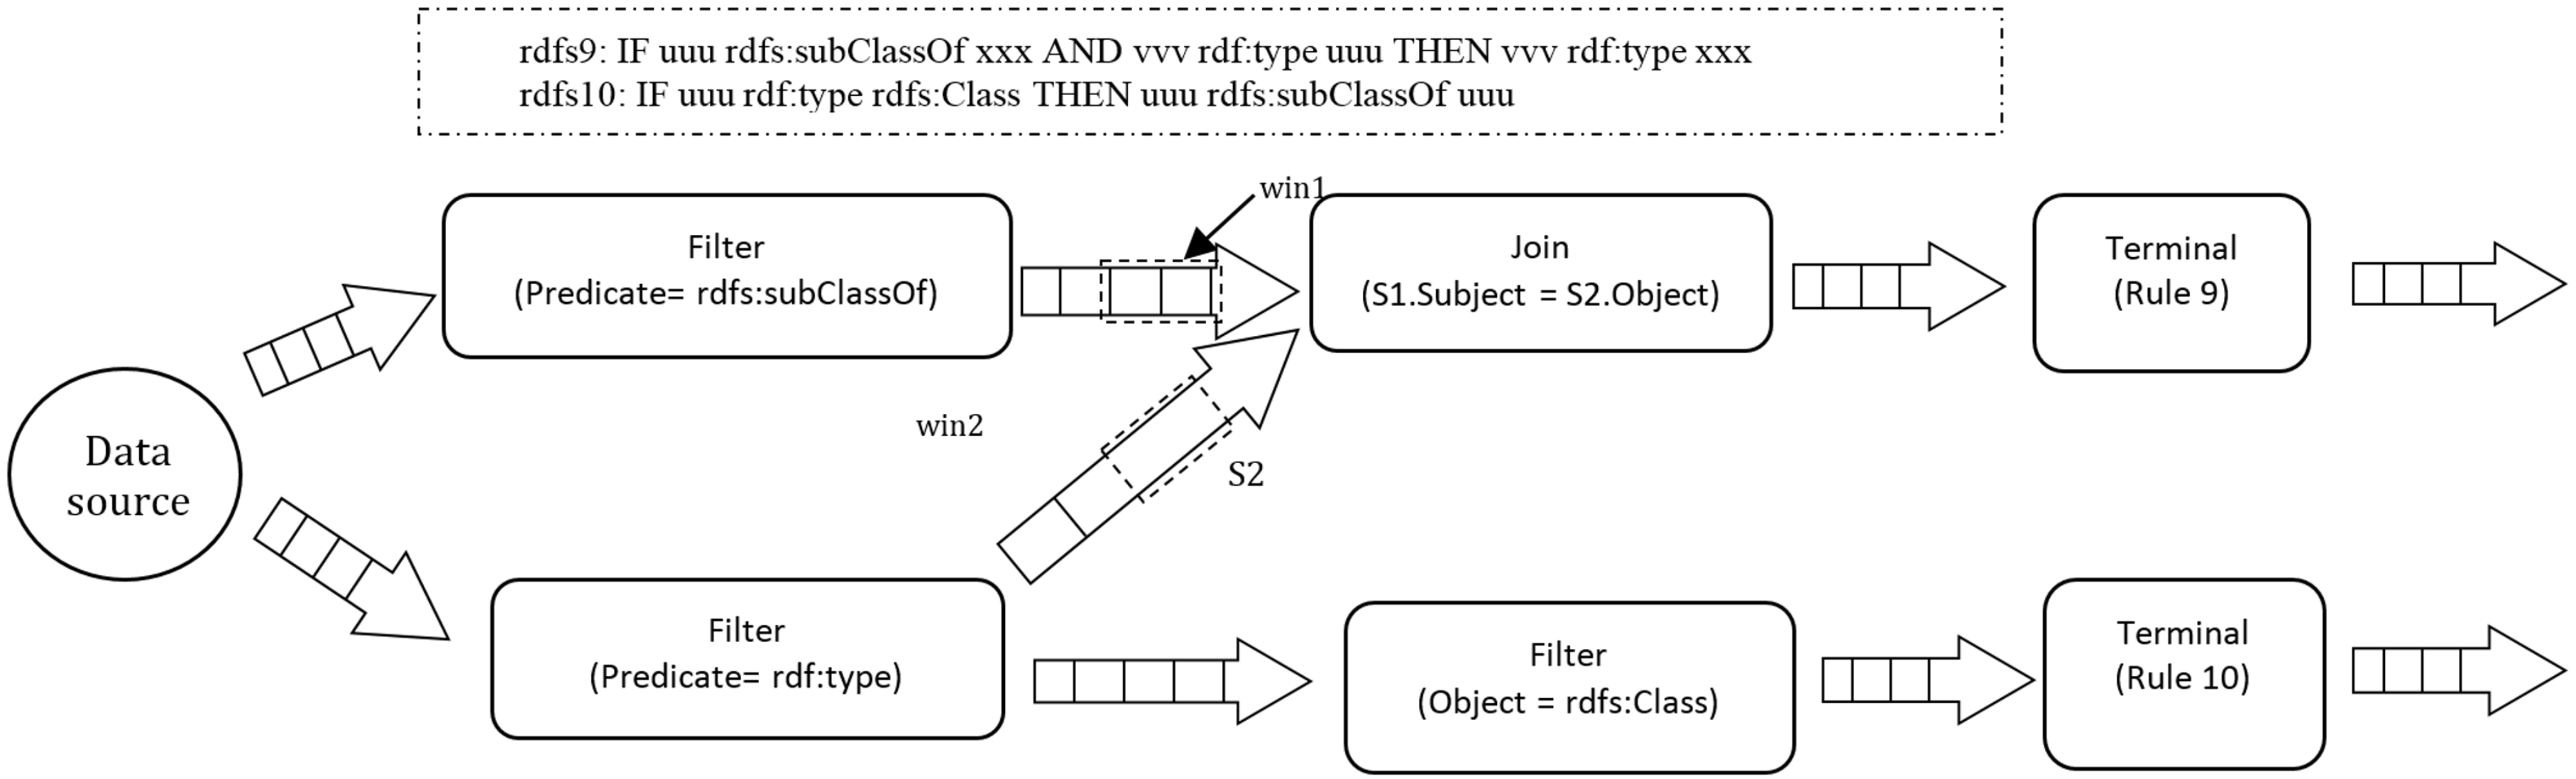
\includegraphics[width=0.9\textwidth]{example-rete-network}
 			\caption{An example Rete network with corresponding (RDFS) rules.}
 			\labelfig{example-rete-network}
 		\end{figure*}
	\end{nestedsection}
\end{nestedsection}
